%TEX root = ../dissertation.tex

\chapter{Solution}
\label{chapter:solution}
% Overview about the solution
% Types of users
% For each one, who he is, what he does...
% What was implemented for each one
The main goal of our solution is to assist
the development proximity-based mobile applications.
There are already some tools available for this purpose (presented in section \ref{sec:background_related_work}).
However, some of them are attached to a given platform, that is, developers
need to write one proximity-based application for each platform they want
to reach.
In order to circumvent this limitation, this solution allows developers
to use the same technologies that are used for any web application, such as \gls{HTML}, \gls{CSS} and Javascript.

Before starting the description of our solution, we need to take a look at three kinds of users that will be part of it:
\begin{description}
  \item[Owners:] These users are the ones responsible for managing a given place that they want to turn into a Smart Place;
  \item[Developers:] The users that develop the code of the Smart Places;
  \item[End users:] Anyone with a mobile device that install an app to scan for nearby Smart Places.
\end{description}

Smart Places solution has a component that targets each one of the presented type of user.
Owners have a mobile app that allow them to turn the places they manage into Smart Places.
There is another mobile app to allow anyone, with a mobile device, such as a smartphone, to use the services provided by Smart Places nearby.
To develop these services our solution offers an \gls{API} that developers can integrate in their web applications to make them react to the presence of the user.

\section{Mobile app for owners}
\label{sec:solution_mobile_app_for_owners}
% Who are the owners
% What are the main features of the app
% Workflow (with some screenshots)
The Smart Place owners manage one or more places where they want to provide some service to visitors, in their mobile devices.
In order to make owners be able to offer this kind of services, an Android app, designed for them, is offered by this solution.
This app offers the folllowing features:
\begin{itemize}
  \item Get a list of all available Smart Places;
  \item Configure an instance of a given Smart Place;
  \item Delete an existing configuration of a given Smart Place;
  \item Update an instance of a given Smart Place;
\end{itemize}

In order to configure a Smart Place, first, owners need to tag physical objects.
They need to deploy beacons in the right places.
Then, they use the mobile app to create an instance of a Smart Place following the steps shown in Figure~\ref{fig:screenshot_ownersapp}:
\begin{itemize}
  \item First, the app shows a list of all available Smart Places;
  \item Then, the owner selects one and he can see a text explaining what that Smart Place is about;
  \item Finnaly, the owner just needs to type a title and a message, that will appear in the users' mobile devices notifications when they are nearby
\end{itemize}

After creating an instance of a Smart Place, the owner needs to configure tags, that is, associate information to the previously deployed beacons.
This information will depend on the Smart Place.
Figure~\ref{fig:screenshot_ownersapp_configure} shows the needed steps to configure tags in an instance of a given Smart Place.
First, the owner selects the instance from the list of instances that he has created.
Then, he has access to an interface where he can manage the existing tags of that Smart Place instance.
This interface is developed by the same developers that create the Smart Place, using the \gls{API} described in section \ref{sec:solution_developers_api}.

\begin{figure}[!ht]
  \centering
    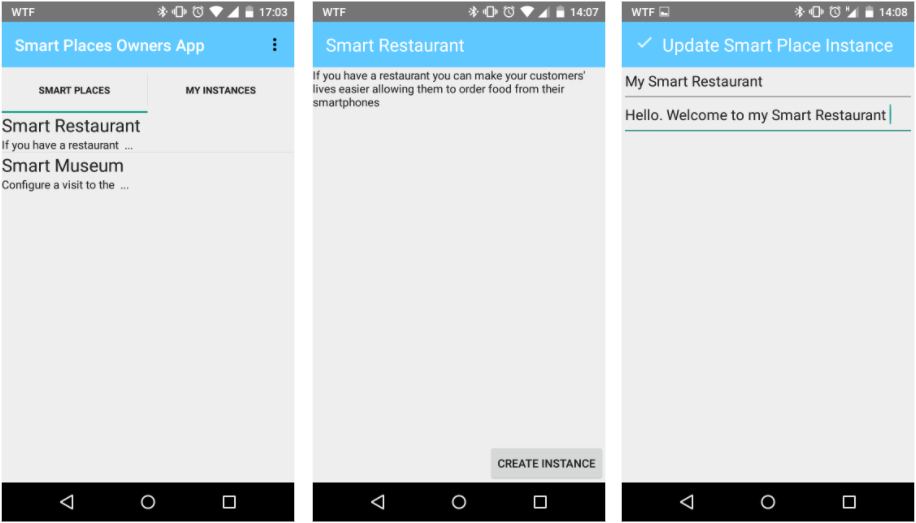
\includegraphics[width=1\textwidth, keepaspectratio]{images/screenshots/ownersapp}
    \caption[Create a Smart Place Instance]{From left to right, the steps to create an instance of a given Smart Place}
    \label{fig:screenshot_ownersapp}
\end{figure}

\begin{figure}[!ht]
  \centering
    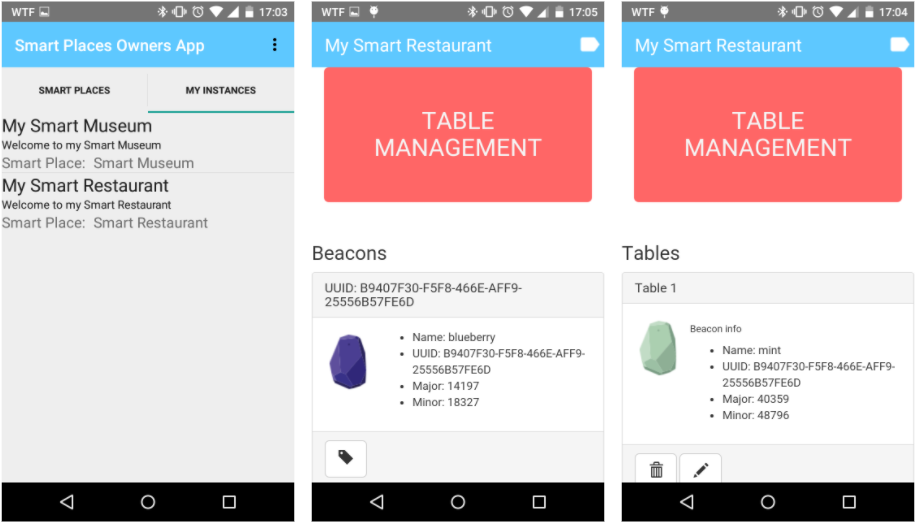
\includegraphics[width=1\textwidth, keepaspectratio]{images/screenshots/ownersapp_configure}
    \caption[Configure a Smart Place Instance]{From left to right, the steps to configure an instance of a given Smart Place}
    \label{fig:screenshot_ownersapp_configure}
\end{figure}

\section{Mobile app for end users}
\label{sec:solution_mobile_app_for_end_users}
% Who are end users
% What are the main features of the app
% Workflow (whith some screenshots)
Anyone that have a mobile device, such as a smartphone, can use the services provided by any Smart Place.
In our solution, there is an Android app, different from the one described in section \ref{sec:solution_mobile_app_for_owners}, that notifies the user when he is nearby any Smart Place.
When the mobile device approaches any Smart Place, the app notifies the user that he is near a Smart Place.
When the user touches these notifications, the app shows an embedded web browser that contains a web page that can react to nearby objects, that is, beacons with meaning to the application.

After installing the app, the first time the user opens it, the app ask the user to turn on the device's bluetooth, as shown in Figure~\ref{fig:screenshot_clientapp_entry}.
\begin{figure}[!ht]
  \centering
    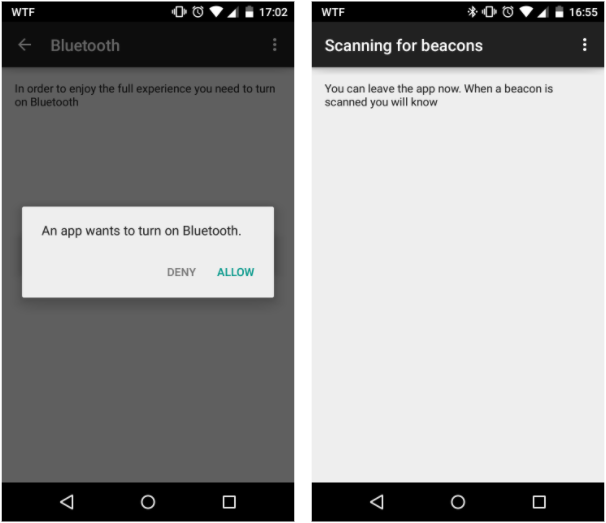
\includegraphics[width=0.7\textwidth, keepaspectratio]{images/screenshots/clientapp_entry}
    \caption[Users mobile app]{First time the user opens the mobile app}
    \label{fig:screenshot_clientapp_entry}
\end{figure}
This app will scan for nearby beacons, periodically.
Each time a beacon is scanned, the app shows a notification associated to a Smart Place.
If the scanning period is small, the app can constantly notify the user. Otherwise, if this period is big, the user will receive less notifications.
According to his preference, our app allows the user to change the scan periods in background and foreground modes.

\section{Developers API}
\label{sec:solution_developers_api}
% Why javascript api
% Who
% How to use it (with some code snippets)
As already mentioned, owners configure the data of a Smart Place; end users, who are anyone with a mobile device and the app, described in section \ref{sec:solution_mobile_app_for_end_users}, can interact with objects nearby.
But, who will add behavior to these Smart Places, this kind of apps that can react to nearby objects with special tags?
Our solution offers a way for developers to create their Smart Places.
Also, we want to avoid the user having to install one mobile app for each Smart Place.
This is way, the app for end users,
has an embedded web browser, so they can use any Smart Place, as they would use any web application, without the need to install one more mobile app.
That is why a Javascript library is part of our solution.
This way, an existing web application can use this library and make it react to nearby objects tagged with \gls{BLE} beacons.

The library was turned into an open-source project, hosted on a github repository\footnote{http://github.com/samfcmc/smartplaces-js} and it is available, to install, using bower\footnote{http://bower.io}, which is a tool to manage frontend dependencies in web applications.
If a developer, wants to install this library, he/she just needs to run the command, as shown in Listing~\ref{code:bower_install}

\begin{listing}[H]
  \begin{minted}{shell}
  bower install smartplaces-js --save
  \end{minted}
  \caption[Install library using Bower]{Command to install smartplaces-js library using bower}
  \label{code:bower_install}
\end{listing}
Then, he/she just needs to include the library and use the available functions.
The library is event-based, that is, the mobile apps, described in sections \ref{sec:solution_mobile_app_for_owners} and \ref{sec:solution_mobile_app_for_end_users}, emit events to the library, such as, a nearby beacon is detected, to the web application running inside a embedded web browser.
In this library, there is a global object, which is ``SmartPlaces'' with several methods.
All those methods need to receive a callback because, as already mentioned, the library follows an event-based approach.
However, developers are also responsible to create the interface to configure the Smart Place, that is, the steps that owners have to follow, as described in section \ref{sec:solution_mobile_app_for_owners}, after they select the Smart Place they want.
In the part of the web app, that will be accessed by owners, developers first need to initialize the library, as shown in Listing~\ref{code:smartplaces_initialization}.
\begin{listing}[H]
  \begin{minted}{javascript}
    SmartPlaces.onInit(function(smartPlaceInstance) {
      // Code after initialization of this Smart Place Instance
    });
  \end{minted}
  \caption[Javascript library initialization]{Javascript library initialization}
  \label{code:smartplaces_initialization}
\end{listing}

When the owner, is using the app, described in section \ref{sec:solution_mobile_app_for_owners}, there is a button that, when is touched, the app scans for nearby beacons and sends an event to the javascript library.
Developers have to define the behaviour, when this event is emitted, as shown in \ref{code:smartplaces_on_beacons_scanned}.

\begin{listing}[H]
  \begin{minted}{javascript}
    SmartPlaces.onBeaconsScanned(function(beacons) {
      // Code to handle beacons that were scanned
    });
  \end{minted}
  \caption[Beacons scanned]{Defining a callback function when beacons are scanned by the mobile app for owners}
  \label{code:smartplaces_on_beacons_scanned}
\end{listing}

The argument named ``beacons'' in callback function in \ref{code:smartplaces_on_beacons_scanned}, it is an array of \gls{JSON} objects, where each one has the following keys:
\begin{itemize}
  \item uuid: The \gls{UUID} of the beacon that was scanned;
  \item major: The major value, according to the ibeacon protocol;
  \item minor: The minor value, according to the ibeacon protocol.
\end{itemize}

However, there is more information about each beacon, for instance, its name and its icon \gls{URL}.
To get this extra information, from a beacon \gls{JSON} object, there is a ``getBeacon'' function, which usage is shown in Listing~\ref{code:smartplaces_get_beacon}.
Since this function makes a request to the backend, we need to pass, as an argument, an object with two keys:
\begin{itemize}
  \item success: Callback function, when the request was successfull made and we got a response with an object that, besides the keys mentioned before, \gls{UUID}, major and minor, we also got the name and icon, which is an \gls{URL} that we can use to get the image of that particular beacon;
  \item error: Callback function, when the request returns an error.
\end{itemize}

\begin{listing}[H]
  \begin{minted}{javascript}
    SmartPlaces.getBeacon(beaconScanned, {
      success: function(beacon) {
        // Code to handle when a beacon object was retrieved successfully from the backend
      },
      error: function(error) {
        // Code to handle when an error occurrs when trying to get a beacon object from the backend
      }
    });
  \end{minted}
  \caption[Get beacon object]{Get beaon info from the backend}
  \label{code:smartplaces_get_beacon}
\end{listing}

After we got the beacon object with all the information, it is possible to associate a \gls{JSON} with any structure.
To do that, there is an ``associateTag'' function, which usage is illustrated in Listing~\ref{code:smartplaces_associate_tag}. We need to pass the beacon object, the object with the data that we want to associate with the beacon, and another object with success and error keys, similar to what is shown in Listing~\ref{code:smartplaces_get_beacon}.

\begin{listing}[H]
  \begin{minted}{javascript}
    SmartPlaces.associateTag(beacon, tagData, {
      success: function(tag) {
        // Code to handle when a tag is successfully associated to a beacon
      },
      error: function(error) {
        // Code to handle when an error occurrs trying to associate a tag to a beacon
      }
    });
  \end{minted}
  \caption[Associate tag]{Associate a tag to a given beacon}
  \label{code:smartplaces_associate_tag}
\end{listing}

It is also possible to update an existing tag. For that, developers can use the ``updateTag'' function. Its usage is shown in Listing~\ref{code:smartplaces_update_tag}. This function require, the existing tag object and an object with success and error keys, similar to the other functions that make requests to the backend.

\begin{listing}[H]
  \begin{minted}{javascript}
    SmartPlaces.updateTag(tag, newData, {
      success: function(updatedTag) {
        // Code to handle when the given tag is successfully updated
      },
      error: function(error) {
        // Code to handle when an error occurrs when trying to update the given tag
      }
    });
  \end{minted}
  \caption[Update an existing tag]{Update data of a given tag}
  \label{code:smartplaces_update_tag}
\end{listing}

The previously mentioned functions, are available in order to make developers able to create the interfaces for owners.
For the end users, the mobile app detects nearby objects and emit an event to the web application, running inside the embedded web browser.
Developers need to define a callback function for this event.
To do that, the ``onTagFound'' can be used, as shown in Listing~\ref{code:smartplaces_tag_found}.
The tag object, which is the argument of this callback function, is the \gls{JSON} object created previously in the code illustrated in Listing~\ref{code:smartplaces_associate_tag}.

\begin{listing}[H]
  \begin{minted}{javascript}
    SmartPlaces.onTagFound(function(tag) {
      // Code to handle when the mobile app detects a tag
    });
  \end{minted}
  \caption[Tag found]{Callback for when a nearby tag is found}
  \label{code:smartplaces_tag_found}
\end{listing}

\section{Examples}
\label{sec:solution_examples}
% Why
% Introduce each one
% Explain the main features
Our solution offers a tool, for developers, to develop Smart Places, that is, proximity-based services, that users can interact with, using their mobile devices.

% Created one example, extracted one API, applied to other example
First, we have created an example of a Smart Place, which is the Smart Restaurant.
While builiding this example, we wrote Javascript code to handle the events emitted by the mobile apps, described in sections \ref{sec:solution_mobile_app_for_owners} and \ref{sec:solution_mobile_app_for_end_users}.
From this code, it was possible to create a library that resulted in a complete independent project, from which, the examples depend on.
After building the first example, we developed another one, which is the Smart Museum.
We defined the Javascript library as a dependency and observed that the same \gls{API} that fits the Smart Restaurant example, also was used in the other example.
Also, we avoided to develop the examples completely from the scratch.
Instead, we tried to integrate the \gls{JS} \gls{API}, described in section \ref{sec:solution_developers_api}, with existing applications or \glspl{API}.

As already mentioned, two examples were created.
The first, described in section \ref{sub:solution_smart_restaurant}, is a Smart Place, for restaurants, to allow customers place their orders without the need to wait.
The other one, is a proximity-based service for museums.
It allows users, that have the mobile app, described in section \ref{sec:solution_mobile_app_for_end_users}, having access to more information about a piece that they are close to, in a museum exhibition.
Its features are described in section \ref{sub:smart_museum}.

\subsection{Smart Restaurant}
\label{sub:solution_smart_restaurant}
The Smart Restaurant is one of the two examples of Smart Places that were created to show the usage of the entire solution.
The main goal here is to allow restaurants' customers to place their orders, using their mobile devices, such as smartphones, without having to wait for an employee coming to them.
When customers arrive at this Smart Restaurant, a notification shows up, in their devices, with a message saying that they can place their orders using the mobile app, such as the one described in section \ref{sec:solution_mobile_app_for_end_users}.
Then, they touch the notification, and a new \gls{UI} appears.
Now, they have access to the restaurant's menu, where they can pick what they want and, in the end, place their orders.
Figure~\ref{fig:smart_restaurant_app}, shows the steps that the customer follows, to place an order, using the mobile app. We can see, from left to right, that, the app detects the table's number and after the sign in, several buttons appear, each one representing a family of products and, in the bottom, there is a button to place the order.
When the customer touches this button, there is a list of the complete order and a button to send the order.

Also, there is a backoffice, where employees and managers, have access to an \gls{UI} to manage the orders and the menu.
This backoffice was implemented in another master thesis\cite{SLOC}.
Our work here, was just to integrate our solution in this backoffice.
There was already an interface to place orders.
We changed this interface to use our Developers \gls{API}, described in section \ref{sec:solution_developers_api} to get the table's number.
We also added an option, to the backoffice's \gls{UI}, to manage the mapping between tables and beacons.

\begin{figure}[!ht]
  \centering
    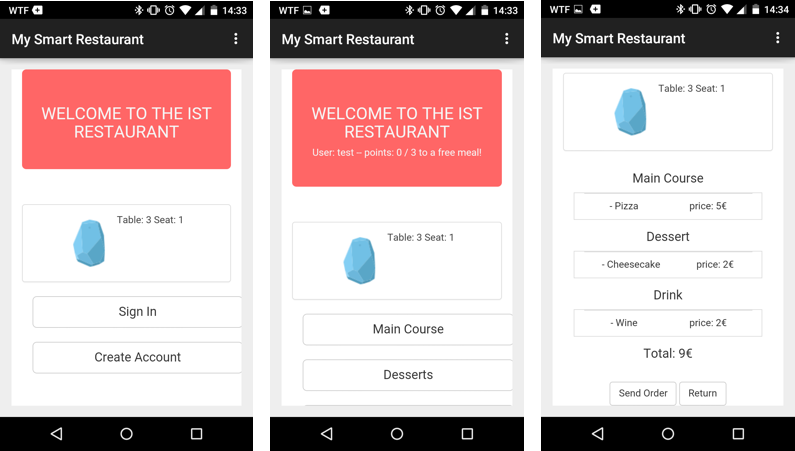
\includegraphics[width=0.8\textwidth, keepaspectratio]{images/screenshots/smart_restaurant_app}
    \caption[Smart Restaurant]{Steps to place an order in the Smart Restaurant app}
    \label{fig:smart_restaurant_app}
\end{figure}

\subsection{Smart Museum}
\label{sub:smart_museum}
The Smart Museum is another example of a Smart Place, that is, a proximity-based service, developed using our solution.
The idea is to allow visitors of a museum, to have access to information, about a given piece, in a given exhibition, in their mobile devices.
Visitors go to the museum and as they look at a given piece, they are notified, through the mobile app, described in section \ref{sec:solution_mobile_app_for_end_users}, that, they can get more information about that.
Then, when they touch in the notification, a screen appears with the information about that piece that they are looking at.
Figure~\ref{fig:smart_museum_app} shows a screen, in the mobile device, after the museum's visitor have touched the notification.

\begin{figure}[!ht]
  \centering
    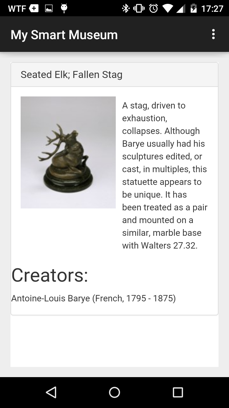
\includegraphics[width=0.4\textwidth, keepaspectratio]{images/screenshots/smart_museum_app}
    \caption[Smart Museum]{Smart Museum app showing information}
    \label{fig:smart_museum_app}
\end{figure}

Instead of creating a fake museum, with mock data, we used real data from a real data source.
The idea was to try to emulate the real experience.
For that, we have used data from the Walters Art Museum\footnote{http://thewalters.org}, which is a public art museum, located in Mount Vernon-Belvedere, Baltimore, Maryland.
It was founded in 1934 and its collection includes more than 30 000 objects.
The way we got the data about the collections and objects is detailed in chapter \ref{chapter:implementation}, section \ref{sub:implementation_smart_museum}.
